\subsection{Reengineered Task Organization Model}
Das Reengineered Task Organization Model repräsentiert die Arbeit des Benutzers mit Hilfe des zu entwickelnden Systems. Die Abbildung \ref{img:reengineeredTaskOrganizationModel}: \glqq \nameref{img:reengineeredTaskOrganizationModel}\grqq{} beschreibt den Prozess der Arbeit des Diabetikers mit dem System anhand von Concrete Use Cases aus der Aufgabenmodellierung und ergänzt das Task Organization Model. Alle Erkenntnisse aus der Aufgabenmodellierung fließen zunächst in das Reengineered Task Organization Model und folglich auch in das Design der Screens ein.
\begin{figure}[H]
	\centering
	\setlength{\fboxsep}{1pt}
	\setlength{\fboxrule}{1pt}
	\fbox{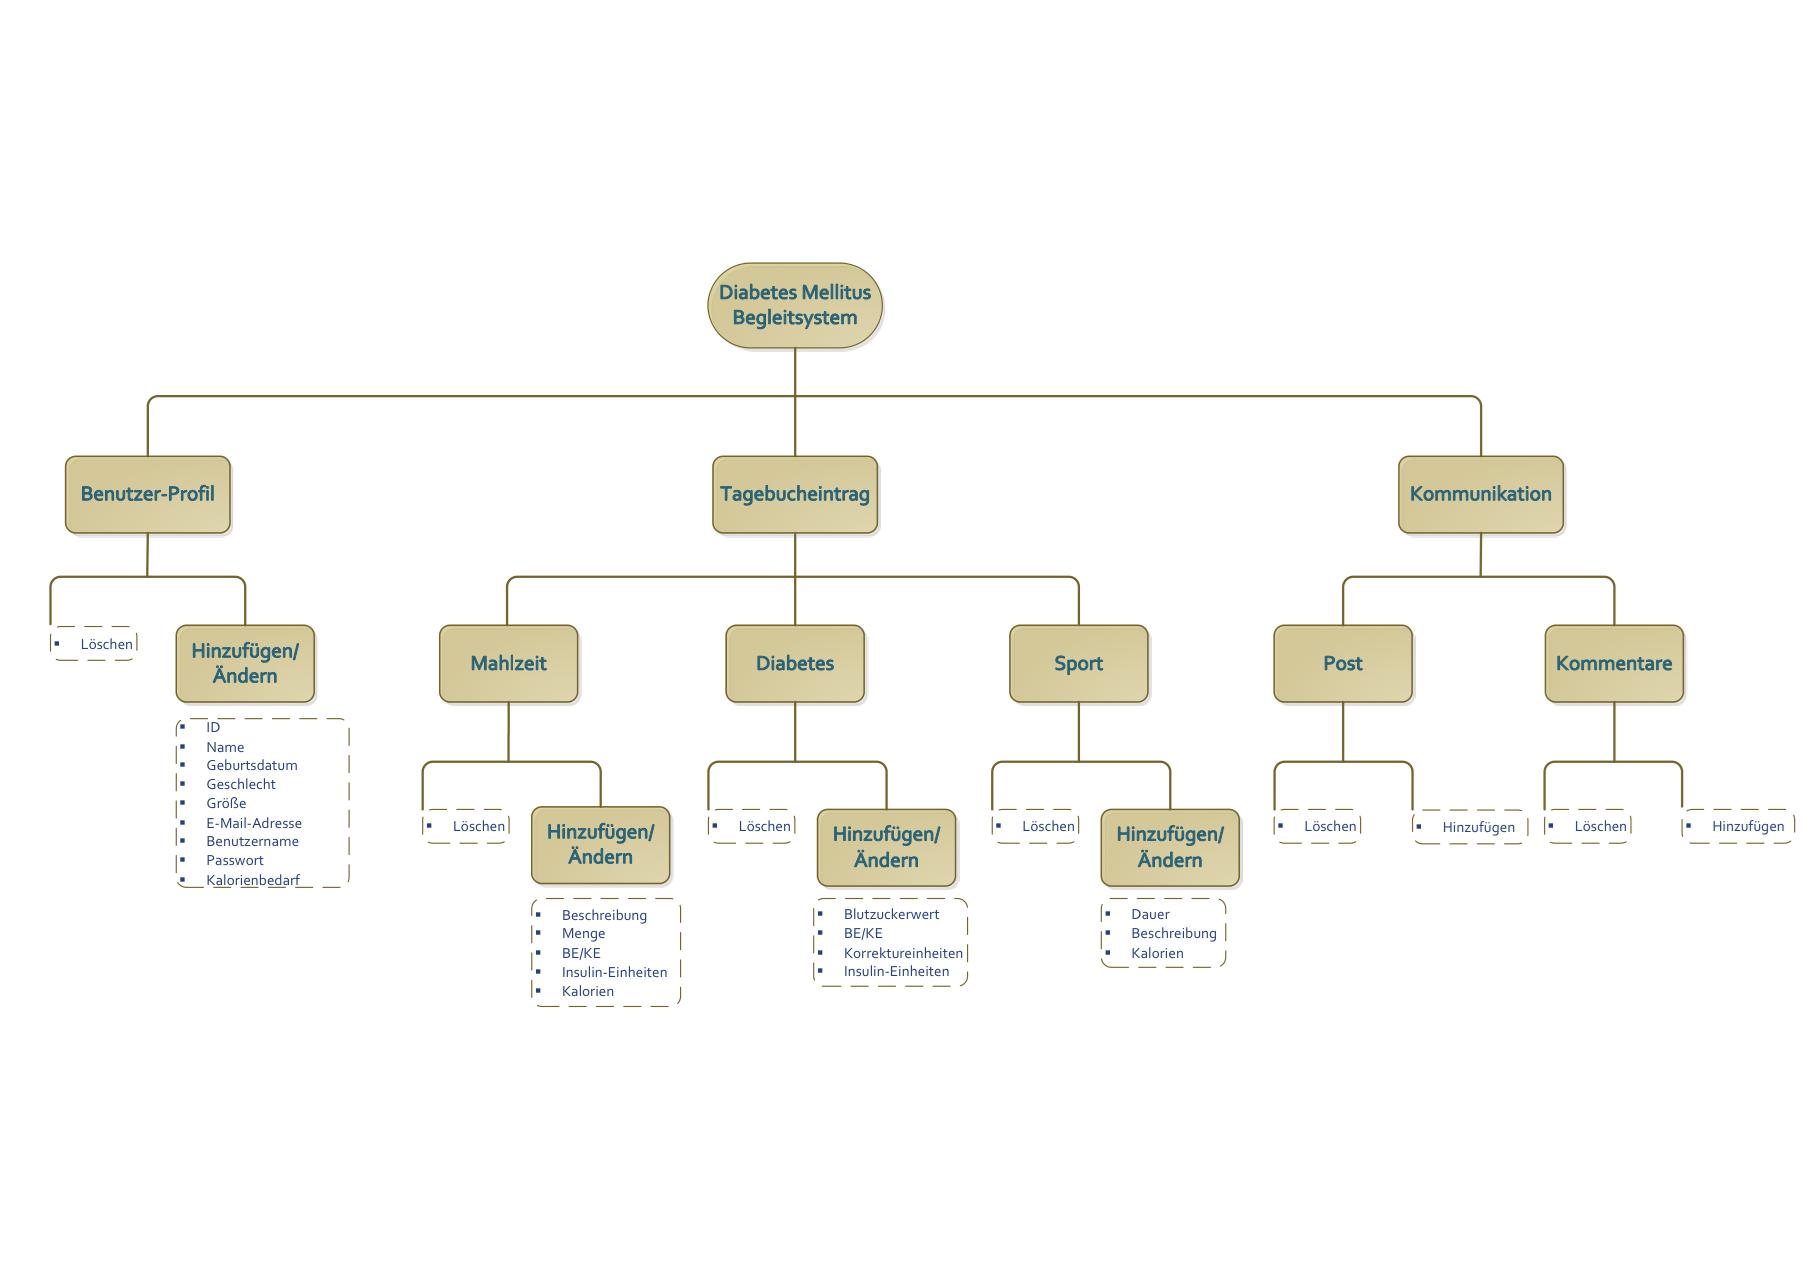
\includegraphics[width=1.0\textwidth]{images/reengineeredTaskOrganizationModel.png}}
	\captionsetup{justification=centering}
	\caption{Reengineered Task Organization Model}
	\label{img:reengineeredTaskOrganizationModel}
\end{figure}
\subsection{Conceptual Model (CM) Design}
Im Conceptual Model Design werden erste Screens für das zu entwickelnde System designt. Die ersten Grobentwürfe sollen den Navigationspfad und die Hauptbildschirme (Main Screens) identifizieren und sie auf der Grundlage der ersten Regeln für die endgültige Gestaltung der Benutzeroberfläche (Interface Design) definieren. Ziel ist es hier jedoch nicht, ein detailreiches Interface-Design zu ermitteln. Dieses Design muss zuerst in den kommenden Entwurfsaufgaben entwickelt werden.\\
Nach Mayhew \cite{MD} muss zunächst festgestellt werden, ob das CM-Design ein product- oder process-oriented model ist, da in dem zu entwickelnden System keine Arbeitsprodukte vorhanden sind, die vom Benutzer individuell erstellt oder bearbeitet werden. In diesem System sollen die Arbeitsprozesse von Diabetikern unterstützt werden.\newline
Alle Benutzer haben Zugriff auf Informationen wie den Nährwert von Lebensmitteln, die abgerufen und im Tagebuch gespeichert werden können. Aus diesem Grund ist dies ein prozessorientiertes Modell (process-oriented model).\\
Der nächste Schritt besteht darin, die Prozesse des process-oriented model zu identifizieren. Dabei definiert das \nameref{img:reengineeredTaskOrganizationModel} (Seite \pageref{img:reengineeredTaskOrganizationModel}) die (Unter-) Prozesse des Systems. Die folgende Aufgabenhierarchie kann daraus abgeleitet werden:\\
Benutzer\newline
\noindent\hspace*{10mm}Benutzer hinzufügen\newline
\noindent\hspace*{10mm}Benutzer bearbeiten\newline
\noindent\hspace*{10mm}Benutzer löschen\newline
Tagebuch\newline
\noindent\hspace*{10mm}Blutzuckerwert\newline
\noindent\hspace*{20mm}Blutzuckerwert hinzufügen\newline
\noindent\hspace*{20mm}Blutzuckerwert bearbeiten\newline
\noindent\hspace*{20mm}Blutzuckerwert löschen\newline
\noindent\hspace*{10mm}Mahlzeit\newline
\noindent\hspace*{20mm}Mahlzeit hinzufügen\newline
\noindent\hspace*{20mm}Mahlzeit bearbeiten\newline 
\noindent\hspace*{20mm}Mahlzeit löschen\newline
\noindent\hspace*{10mm}Aktivität\newline
\noindent\hspace*{20mm}Aktivität hinzufügen\newline
\noindent\hspace*{20mm}Aktivität bearbeiten\newline
\noindent\hspace*{20mm}Aktivität löschen\newline
Kommunikation\newline
\noindent\hspace*{10mm}Beitrag\newline
\noindent\hspace*{20mm}Beitrag hinzufügen\newline
\noindent\hspace*{20mm}Beitrag löschen\newline
\noindent\hspace*{10mm}Kommentar\newline
\noindent\hspace*{20mm}Kommentar hinzufügen\newline
\noindent\hspace*{20mm}Kommentar löschen\\
Eine Bottom-Navigation-Bar wird verwendet, um die Darstellungsregeln für die Prozesse einzuhalten. Die Navigation könnte wie in Abbildung \ref{img:navigationbar}: \glqq \nameref{img:navigationbar}\grqq{} dargestellt aussehen. Sie wurde ausgewählt, um dem Benutzer die Kontrolle über das System und einige Freiheiten zu geben.\newline
Der Benutzer hat die Möglichkeit, bei versehentlichem Auswählen eines Navigationspfades einen deutlich gekennzeichneten \glqq Notausgang\grqq{} zu wählen und die unerwünschte Systemfunktion über die Navigationsleiste zu verlassen, ohne einen erweiterten Dialog durchlaufen zu müssen.
\begin{figure}[H]
	\centering
	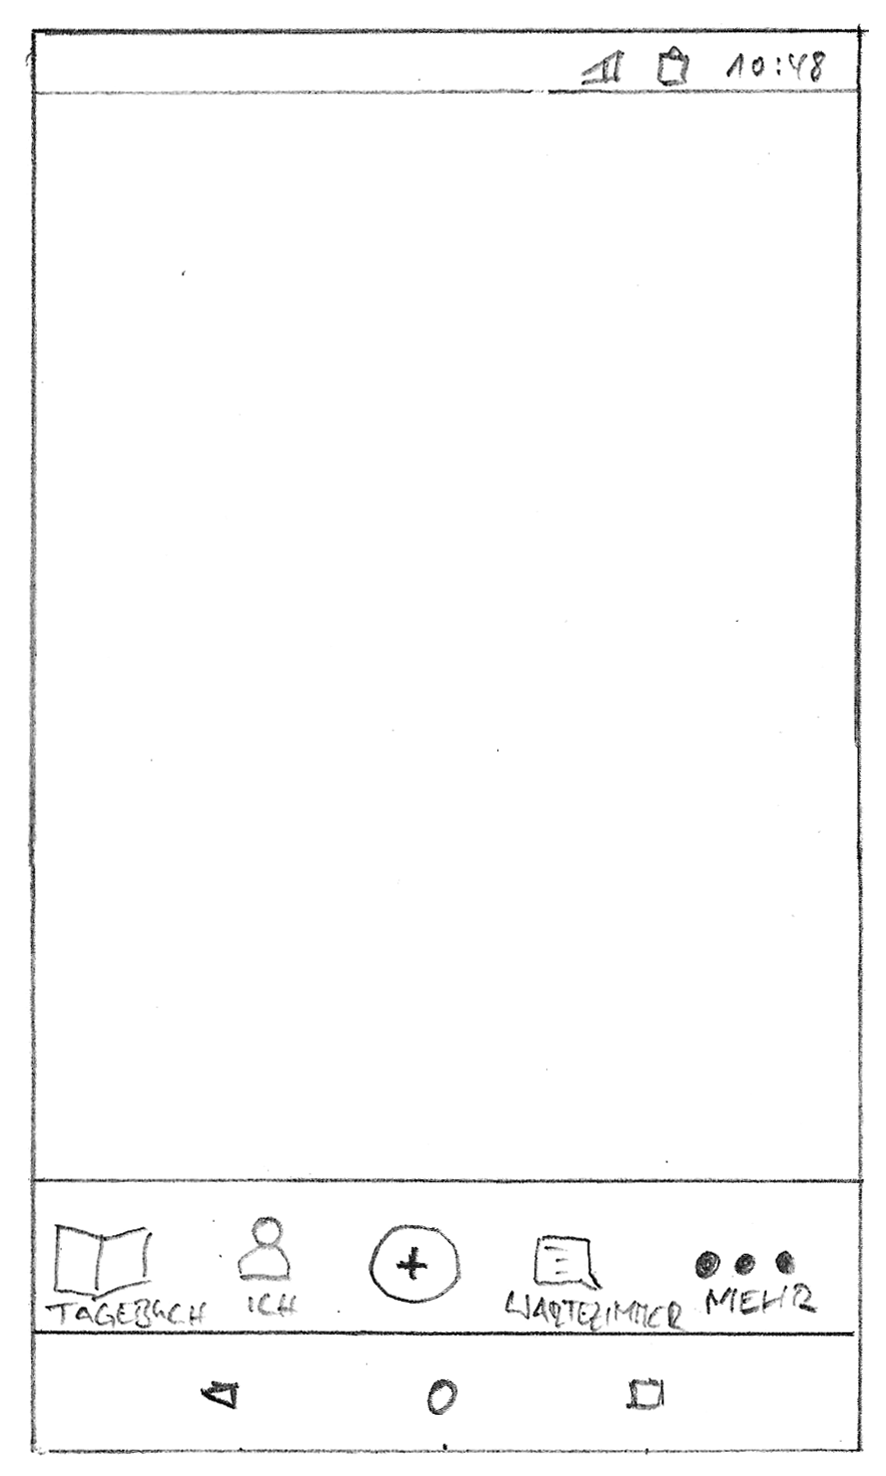
\includegraphics[width=0.35\textwidth]{images/navigationbar.png}
	\captionsetup{justification=centering}
	\caption{Bottom-Navigation-Bar}
	\label{img:navigationbar}
\end{figure}
Unter dem Navigationspfad \glqq Tagebuch\grqq{} (Abbildung \ref{img:tagebuchscreen}: \glqq \nameref{img:tagebuchscreen}\grqq{}) können Blutzuckerwerte, Mahlzeiten und Aktivitäten eingetragen, bearbeitet, angezeigt und gelöscht werden. Benutzerkonten können unter \glqq Ich\grqq{} (Abbildung \ref{img:ichscreen}: \glqq \nameref{img:ichscreen}\grqq{}) und \glqq Mehr\grqq{} (Abbildung \ref{img:mehrscreen}: \glqq \nameref{img:mehrscreen}\grqq{}) angezeigt, bearbeitet und gelöscht werden. Im \glqq Wartezimmer\grqq{} (Abbildung \ref{img:wartezimmerscreen}: \glqq \nameref{img:wartezimmerscreen}\grqq{}) können Beiträge und Kommentare angezeigt, hinzugefügt und gelöscht werden. Mit dem Plus-Icon kann der Anwender auch Blutzuckerwerte, Mahlzeiten, Aktivitäten und Beiträge hinzufügen. Die Screens könnten wie folgt angezeigt werden:
\begin{figure}[H]
	\centering
	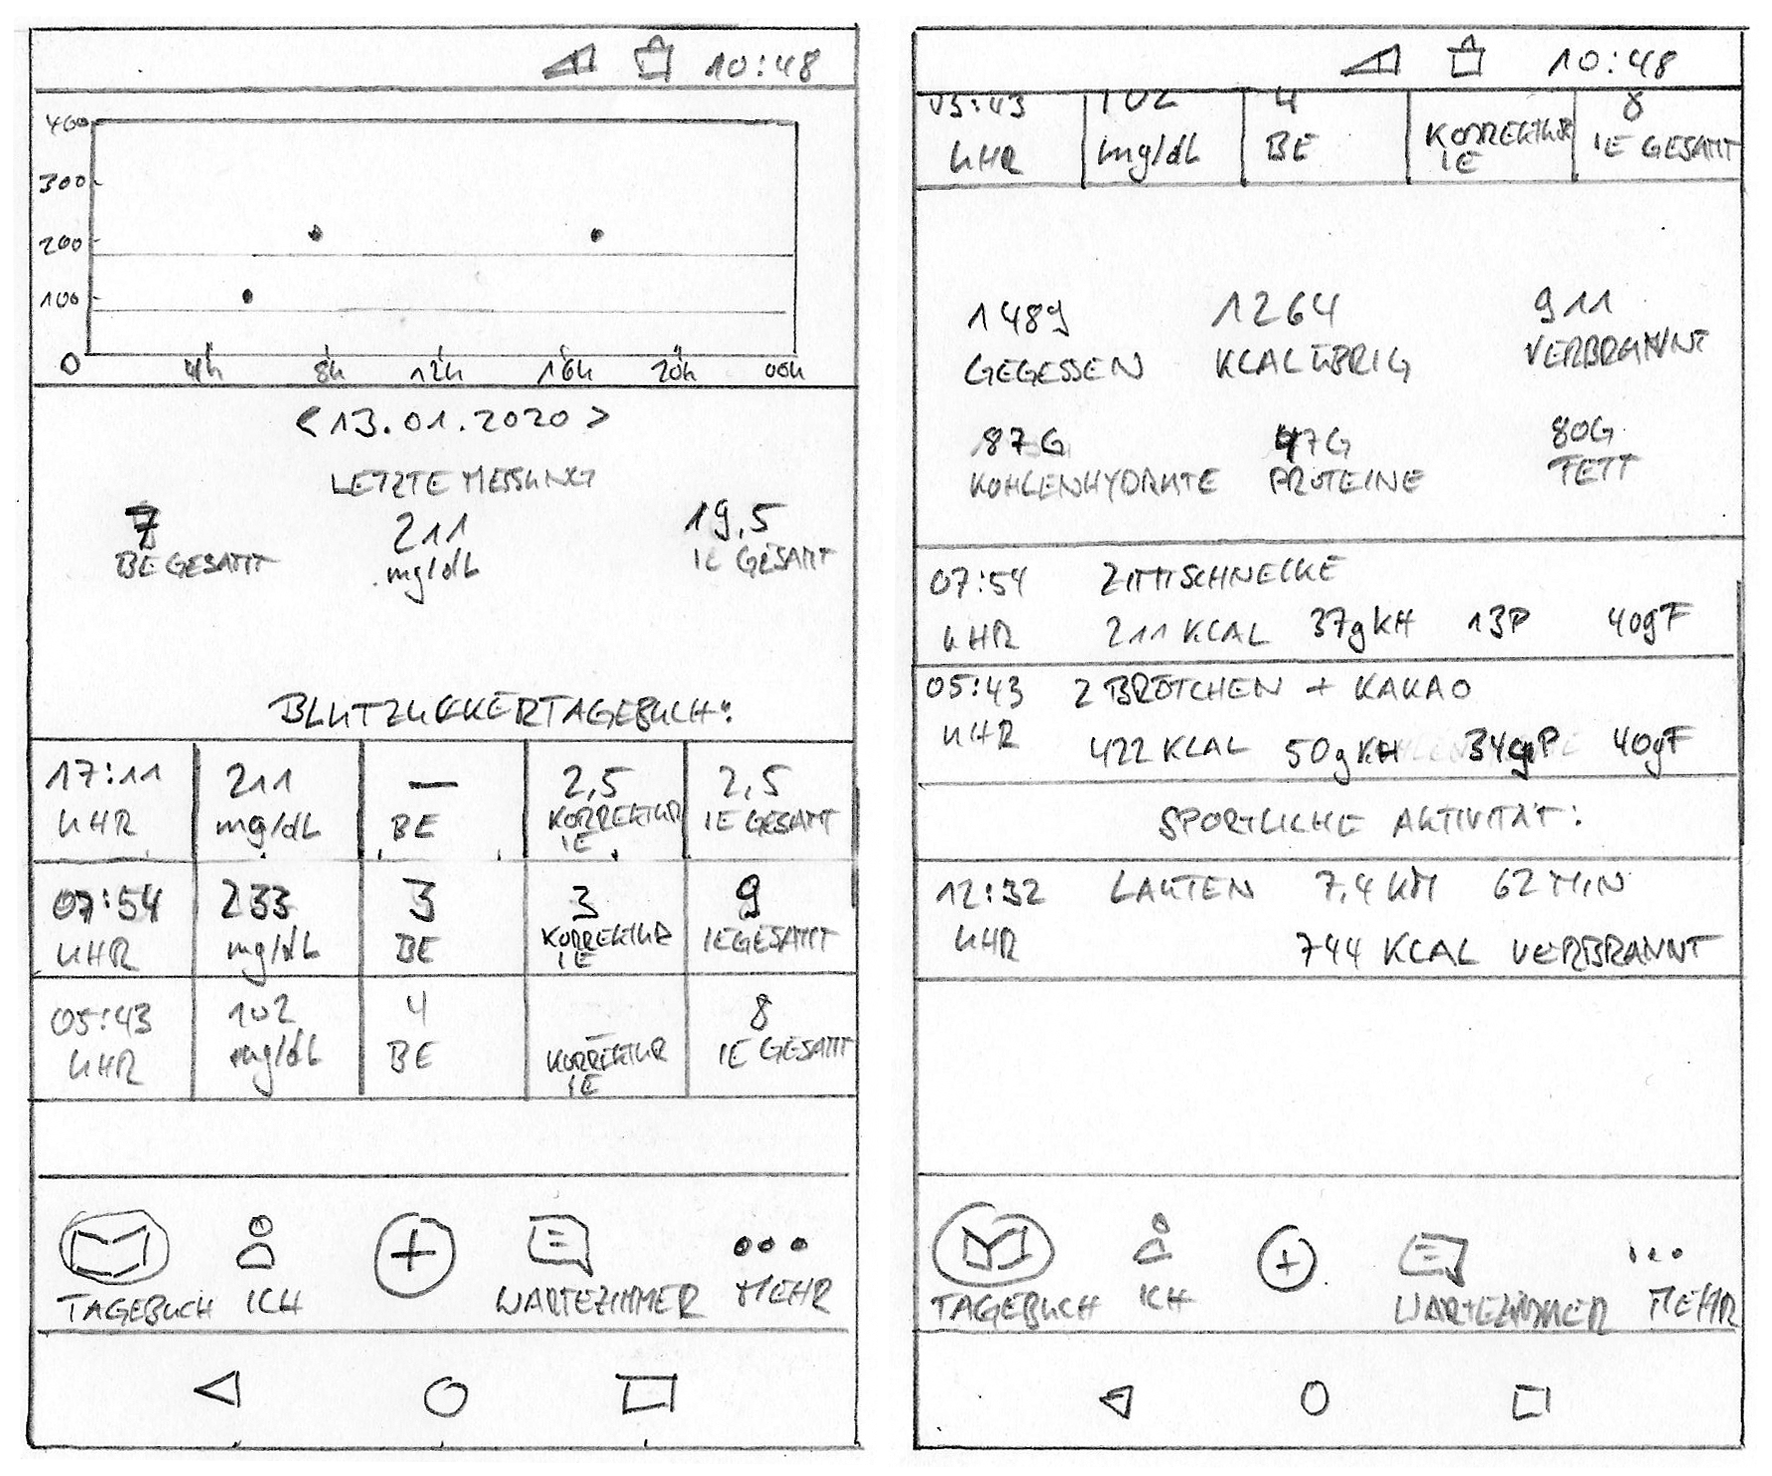
\includegraphics[width=0.66\textwidth]{images/tagebuchscreen.png}
	\captionsetup{justification=centering}
	\caption{Tagebuch-Screen}
	\label{img:tagebuchscreen}
\end{figure}
\begin{figure}[H]
	\centering
	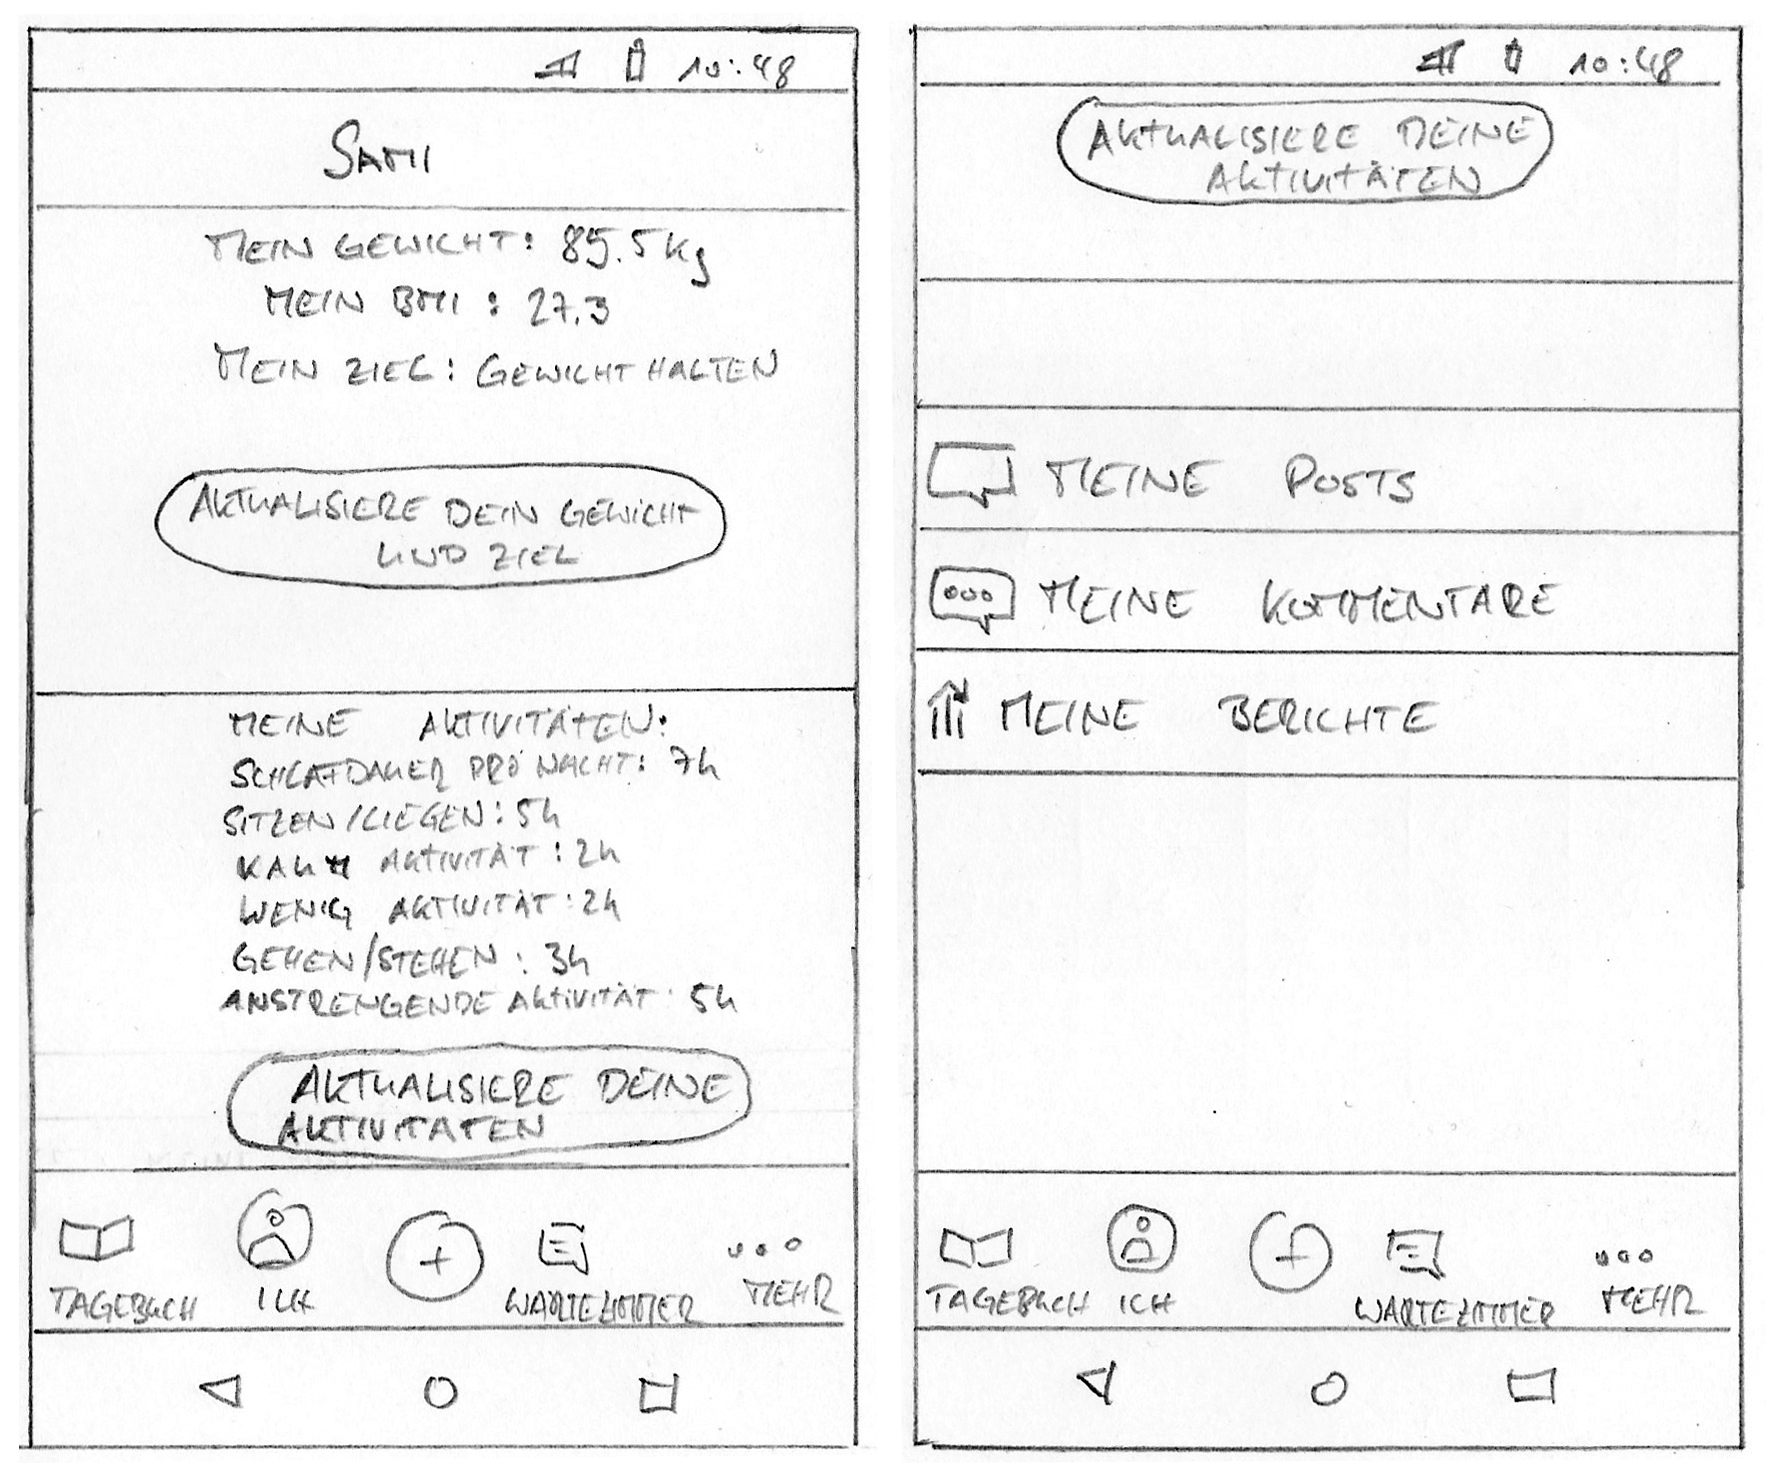
\includegraphics[width=0.66\textwidth]{images/ichscreen.png}
	\captionsetup{justification=centering}
	\caption{Ich-Screen}
	\label{img:ichscreen}
\end{figure}
\begin{figure}[H]
	\centering
	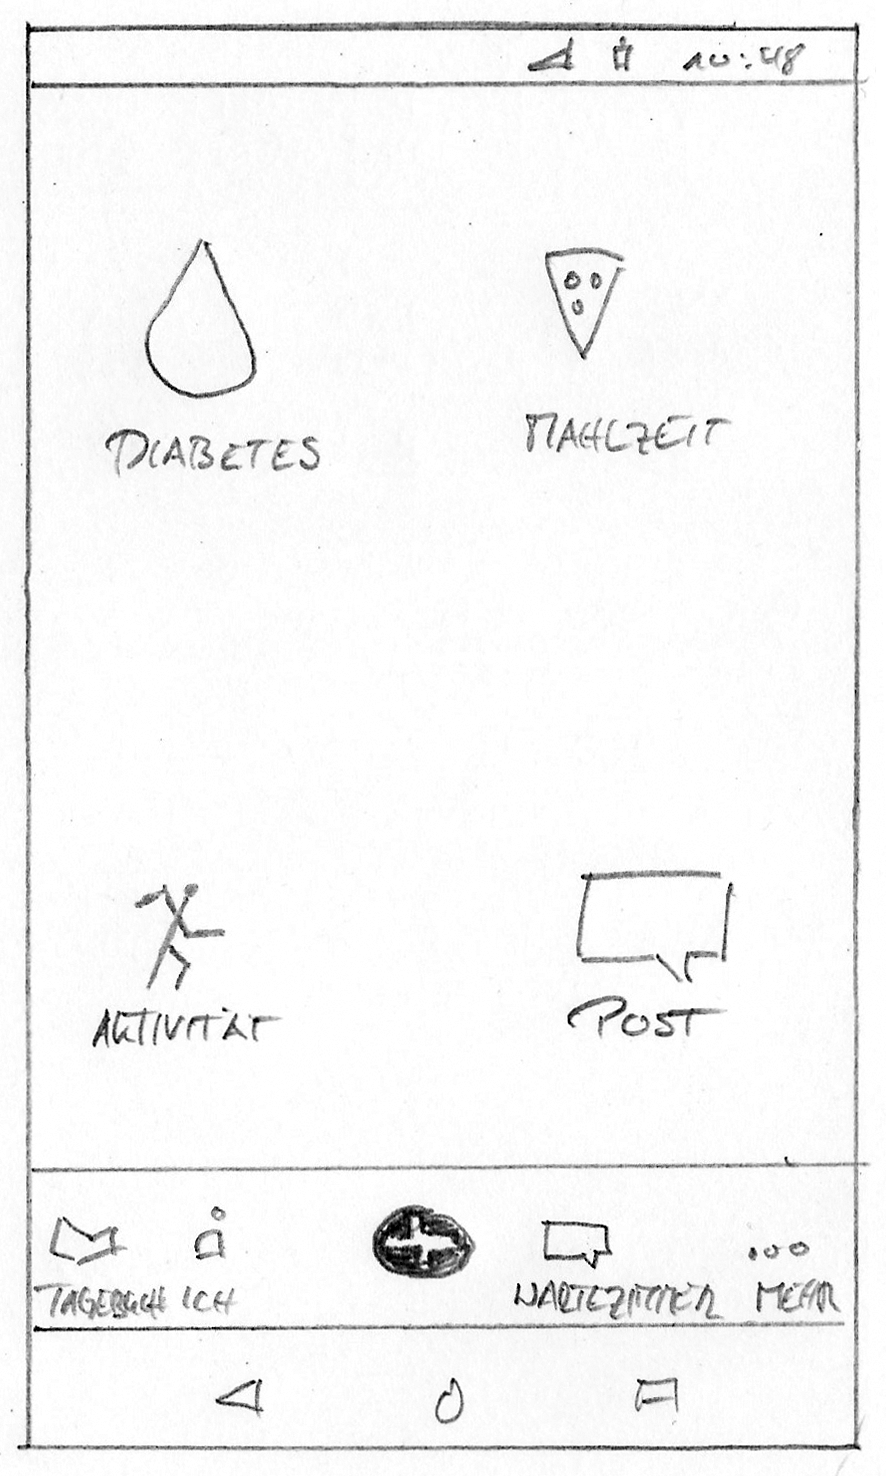
\includegraphics[width=0.33\textwidth]{images/addscreen.png}
	\captionsetup{justification=centering}
	\caption{Add-Screen}
	\label{img:addscreen}
\end{figure}
\begin{figure}[H]
	\centering
	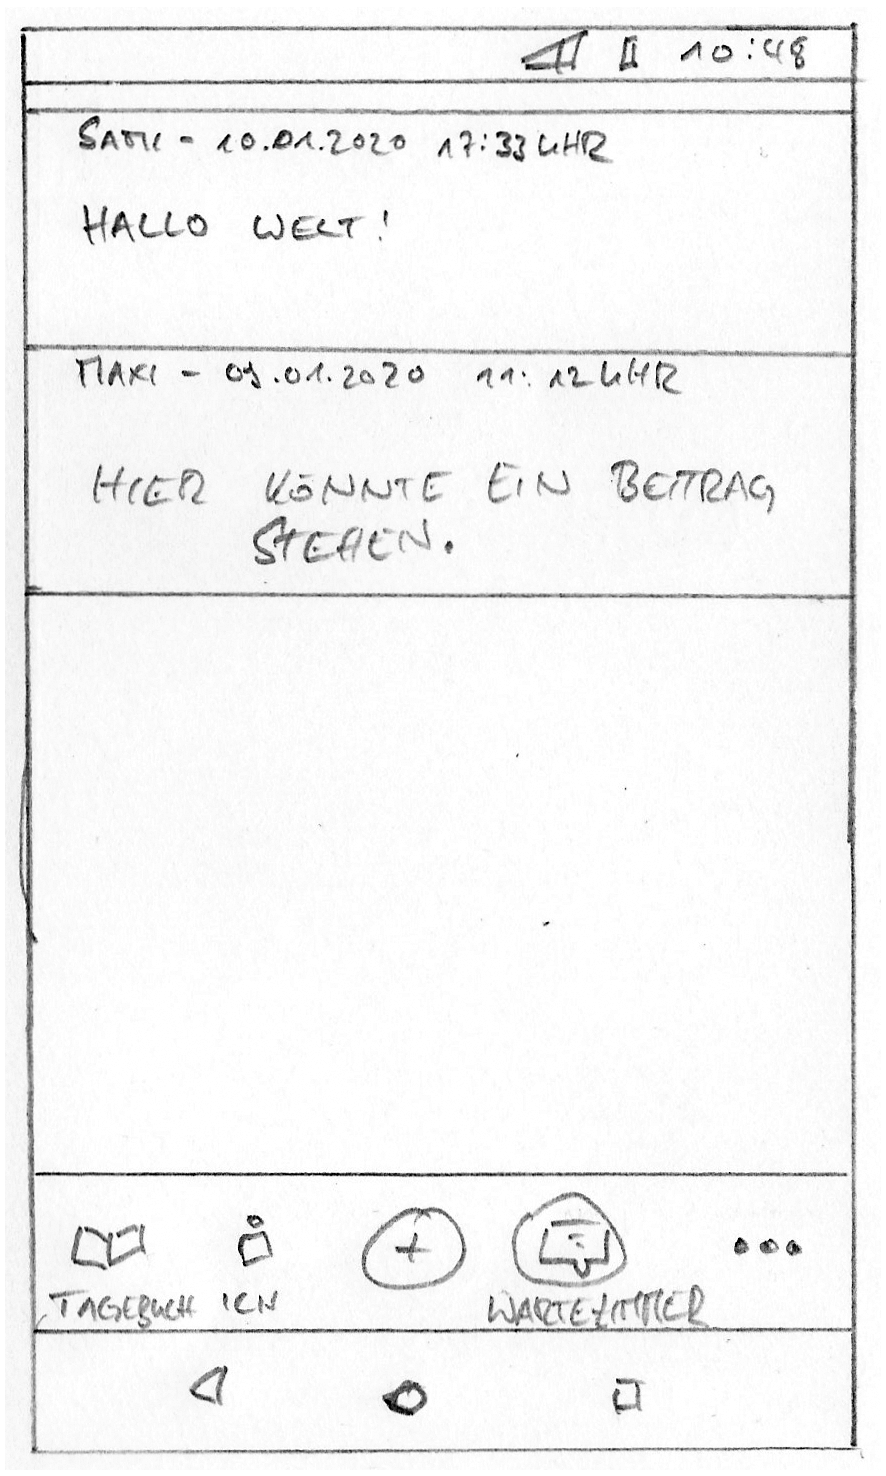
\includegraphics[width=0.33\textwidth]{images/wartezimmerscreen.png}
	\captionsetup{justification=centering}
	\caption{Wartezimmer-Screen}
	\label{img:wartezimmerscreen}
\end{figure}
\begin{figure}[H]
	\centering
	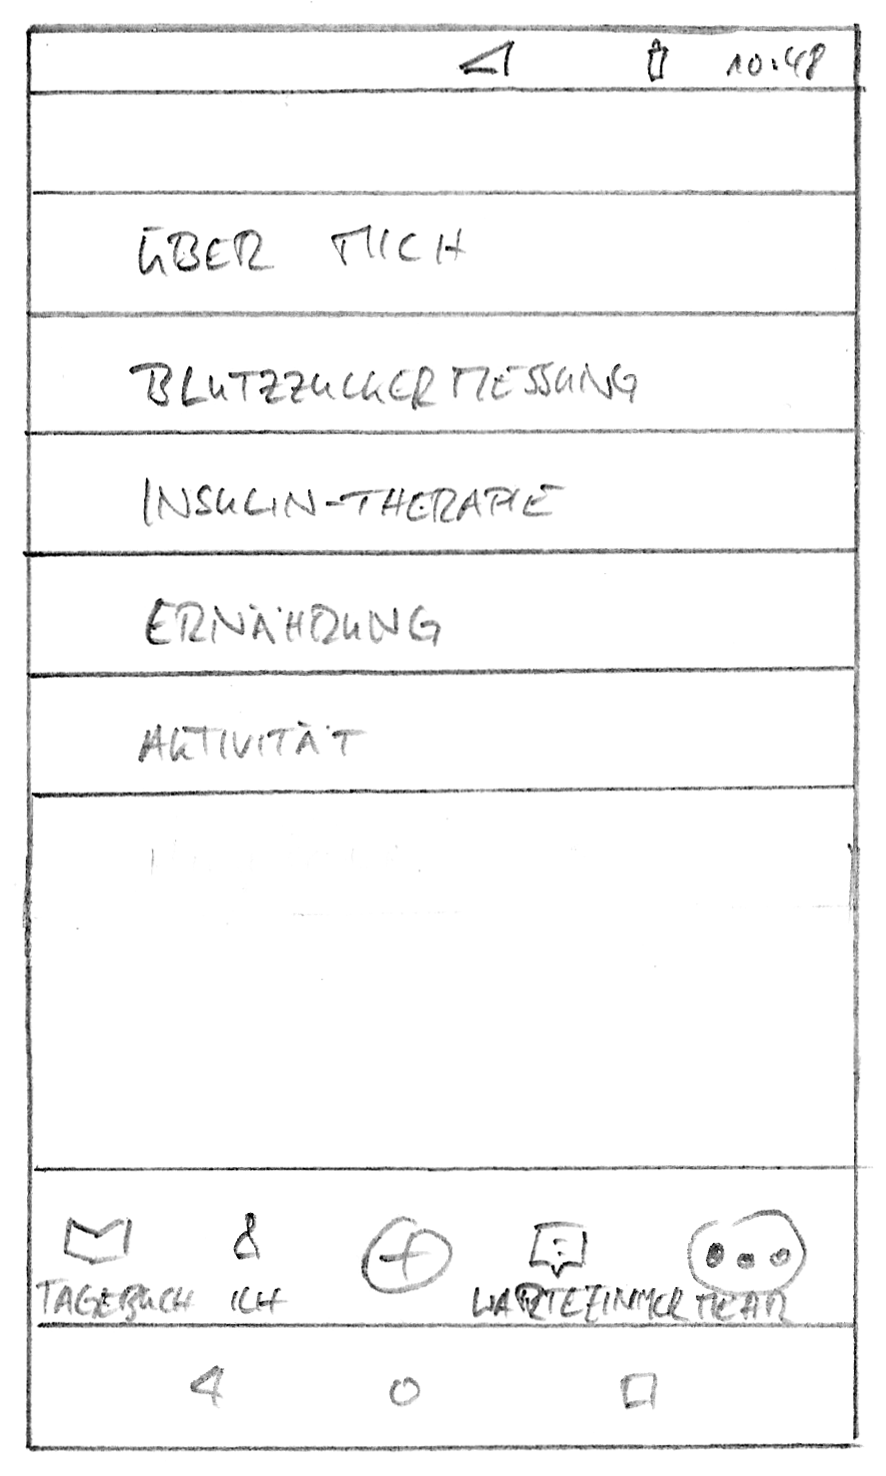
\includegraphics[width=0.33\textwidth]{images/mehrscreen.png}
	\captionsetup{justification=centering}
	\caption{Mehr-Screen}
	\label{img:mehrscreen}
\end{figure}
Der Begriff \glqq Tagebuch\grqq{} (Abbildung \ref{img:tagebuchscreen}: \glqq \nameref{img:tagebuchscreen}\grqq{}) wurde gewählt, weil er in der Diabetiker-Domäne sehr verbreitet ist. Diabetiker machen permanente \glqq Tagebucheinträge\grqq{}. \glqq Ich\grqq{} (Abbildung \ref{img:ichscreen}: \glqq \nameref{img:ichscreen}\grqq{}) kennzeichnet benutzerbezogene Daten recht gut und \glqq Wartezimmer\grqq{} (Abbildung \ref{img:wartezimmerscreen}: \glqq \nameref{img:wartezimmerscreen}\grqq{}) ist eine metaphorische Bezeichnung für einen Treffpunkt verschiedener Benutzer. Unter \glqq Mehr\grqq{} (Abbildung \ref{img:mehrscreen}: \glqq \nameref{img:mehrscreen}\grqq{}) lassen weitere benutzerbezogene Einstellungen bearbeiten. \\
Die verschiedenen Navigationspfade sollen den Benutzer durch entsprechende Informationen in angemessener Zeit auf dem Laufenden halten.\\
Dem oben genannten konzeptuellen Modellentwurf (Conceptual Model Design) folgen das Conceptual Model Mock-Up und die iterative konzeptuelle Modellbewertung (Iterative Conceptual Model Evaluation), in denen die ersten Entwürfe eines Designs mit Stift und Papier erstellt und von Testpersonen bewertet (Evaluation) werden. Aufgrund des begrenzten Zeitrahmens können diese beiden Arbeitsschritte nicht ausgeführt werden, weshalb die Abbildungen ohne Evaluation als Mock-up dienen. Folglich werden die Screen Design Standards festgelegt und daraus ein Style-Guide erstellt.
\subsection{Screen Design Standards (SDS)}
Mithilfe der aus der Benutzer- und Aufgabenmodellierung gewonnenen Erkenntnisse und des Conceptual Model Designs werden systemspezifische Standards und Konventionen für alle Aspekte des detaillierten Screen-Designs entwickelt. Die Standards für das Bildschirmdesign (Screen Design Standards) dienen als Grundlage für die Benutzerfreundlichkeit (Usability) auf der gesamten Benutzeroberfläche (User Interface). Das zu entwickelnde System sollte die folgenden Steuerungs- und Dialogfeldstandards (Control und Dialog Box Standards) erfüllen:\\
\centerline{\textbf{Control Standards}}
\begin{center}
	\begin{longtable}[H]{p{8cm}p{6cm}}
		\textbf{Menu Contents} & \textbf{Control}\\
		\toprule
		Navigationsaktionen & Icon Buttons\\
		Eingabe von Zahlen & EditText mit möglicher Eingabe von Zahlen/Seekbar\\
		Eingabe von Dezimalzahlen & EditText mit möglicher Eingabe von Dezimalzahlen/Seekbar\\
		Eingabe von Text & EditText mit Auswahl von Buchstaben\\
		Auswahl eines Datums & DatePickerDialog\\
		Auswahl einer Uhrzeit & TimePickerDialog\\
		Liste mit Variablen & Spinner/RecyclerView und CardView\\
		\bottomrule
		\captionsetup{justification=centering}
		\caption{Control Standards}
		\label{tab:controlstandars}
	\end{longtable}
\end{center}
\centerline{\textbf{Dialog Box Standards}}
\begin{itemize}
	\item Alle Dialogfelder haben einen blauen Hintergrund.
	\item Titel der Menüleisten, die aufgerufen wurden, werden linksbündig in der Titelleiste geordnet.
	\item Vertikale Gruppen logisch zusammengehöriger Felder.
	\item Zentrierte Ausrichtung von Beschriftungen in Feldgruppen und Feldern, wobei Leerraum zwischen Beschriftungen und Feldern minimiert und Großbuchstaben für alle Hauptwörter in Beschriftungen verwendet werden.
\end{itemize}
Unter Berücksichtigung der Anforderungen dieser Standards könnten die Dialogfelder (Dialog Boxes) wie in Abbildung \ref{img:dialogbox}: \glqq \nameref{img:dialogbox}\grqq{} dargestellt aussehen.
\begin{figure}[H]
	\centering
	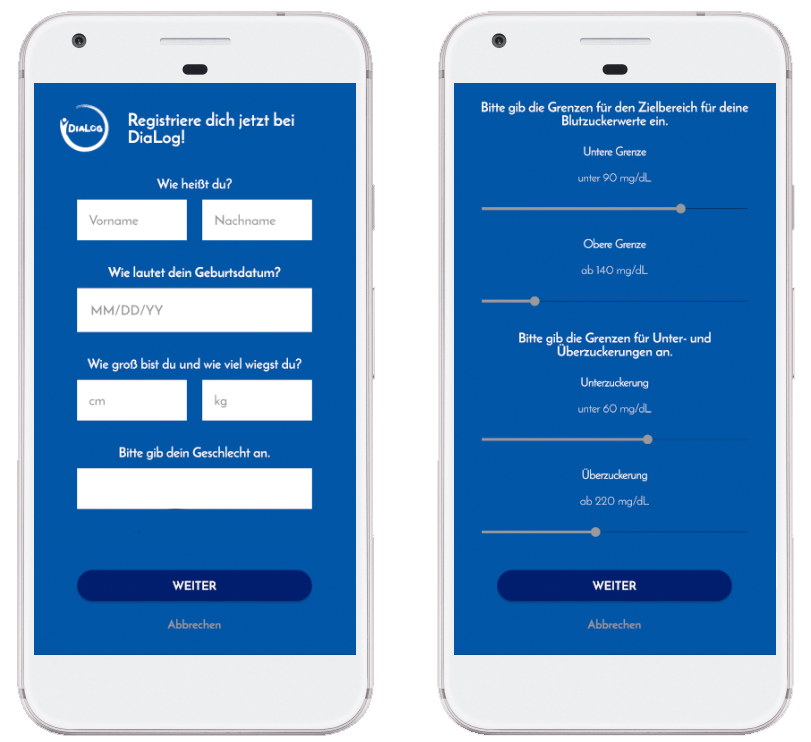
\includegraphics[width=0.66\textwidth]{images/DialogBox.png}
	\captionsetup{justification=centering}
	\caption{Dialog Boxes}
	\label{img:dialogbox}
\end{figure}
Hinzu kommen folgende Standards:
\begin{itemize}
	\item Verwendung von Gruppenfeldern und Einbettung von Titeln mit Großbuchstaben in der oberen Mitte des Gruppenfeldes.
	\item Gruppierte boxes von links nach rechts und von oben nach unten entsprechend der natürlichen Reihenfolge oder der erwarteten Verwendungshäufigkeit geordnet.
	\item \glqq Weiter\grqq{} push button immer in der unteren Mitte und über dem \glqq Abbrechen\grqq{} push button platziert, wobei alle push buttons gleichmäßig voneinander entfernt sind.
	\item Hintergrundfarbe für Eingabefelder:\newline
		\noindent\hspace*{10mm}Read-only - blau \newline
		\noindent\hspace*{10mm}Erforderlich - weiß \newline
		\noindent\hspace*{10mm}Optional - grau 
\end{itemize}
\newpage
\subsection{Style Guide}
Um nun die Screen Design Standards zu vervollständigen, wird ein Style Guide erstellt. Dieser fügt dem User Interface folgende Kriterien hinzu:
\begin{itemize}
	\item Das zu entwickelnde System wird für die Plattform Android entwickelt und soll mit allen Betriebssystemen, höher als Android 7.0 Nougat, kompatibel sein.
	\item Die Displaygröße des Endgerätes muss mindestens 5 Zoll groß sein.
	\item Blau ist die Primärfarbe und Hellblau ist die Sekundärfarbe. Um Akzente zu setzen, wird ein Grauton verwendet. Der Hintergrund für Text- und Eingabefelder ist grundsätzlich weiß.
	\item Als Eingabegerät dient die virtuelle Bildschirmtastatur des Endgerätes mit Touchscreen-Gesten.
	\item Alle Texte erscheinen in der Schriftart \glqq Family Josefin Sans\grqq{}. Die verschiedenen Textarten erfüllen folgende Kriterien:\newline
	\noindent\hspace*{10mm}1. Überschrift: 22dp und Bold\newline 
	\noindent\hspace*{10mm}2. Überschrift: 17dp und Semibold\newline 
	\noindent\hspace*{10mm}Text: 15dp und Light\newline
	\noindent\hspace*{10mm}Hinttext von EditText: 17dp und Semibold\newline
	\noindent\hspace*{10mm}Buttons: 15dp und Bold\newline 
	\noindent\hspace*{10mm}Klickbare Texte: 15dp und Bold 
	\item Buttons und Menüpunkte sollen mit Objekten wie einem Buchsymbol für das Tagebuch, versehen werden, um den kognitiven Arbeitsaufwand des Benutzers zu verringern.
	\item Interaktionen vom Benutzer soll sich das System merken können, damit bei der Suche nach einem Lebensmittel das zuletzt verwendete Lebensmittel vorgeschlagen wird.
	\item Dem Benutzer sollten nach Möglichkeit Eingaben vorgegeben werden. So können beispielsweise BE/KE oder Insulineinheiten vorberechnet werden und bei der Eingabe von Uhrzeiten und Daten werden die aktuellen Parameter vorgeschlagen. Der Benutzer sollte jedoch weiterhin in der Lage sein, sie anzupassen.
	\item Der Benutzer sollte sich keine Informationen von einem Teil eines Dialogs zum nächsten merken müssen.
	\item Der Benutzer sollte immer zum vorherigen Layout zurückkehren können.
\end{itemize}
Das detaillierte Design der Benutzeroberfläche (Detailed User Interface Design) kann nun mit Hilfe der festgelegten Screen Design Standards und des definierten Style Guides entworfen werden.
\subsection{Detailed User Interface Design (DUID)}
	Das Detailed User Interface Design ist das endgültige Design der Benutzeroberfläche. Die bisherigen Ergebnisse aus der Benutzer- und Aufgabenmodellierung, dem Conceptual Model Design, den Screen Design Standards und dem Style-Guide fließen alle in das detaillierte Design der Benutzeroberfläche (Detailed User Interface Design) ein.\newline
	Das System wird wie folgt mit fünf verschiedenen main screens implementiert:
\begin{itemize}
	\item Tagebuch-Screen (Abbildung \ref{img:DUIDtagebuchscreen}: \glqq \nameref{img:DUIDtagebuchscreen}\grqq{})
	\item Ich-Screen (Abbildung \ref{img:DUIDichscreen}: \glqq \nameref{img:DUIDichscreen}\grqq{})
	\item Add-Screen (Abbildung \ref{img:DUIdreiscreen}: \glqq \nameref{img:DUIdreiscreen}\grqq{})
	\item Wartezimmer-Screen (Abbildung \ref{img:DUIdreiscreen}: \glqq \nameref{img:DUIdreiscreen}\grqq{})
	\item Mehr-Screen (Abbildung \ref{img:DUIdreiscreen}: \glqq \nameref{img:DUIdreiscreen}\grqq{})
\end{itemize}
Die folgenden Änderungen wurden am Konzeptmodelldesign (CM Design) vorgenommen:
\begin{itemize}
	\item Jeder Screen hat einen Titel, sodass der Benutzer jederzeit sehen kann, auf welchem Bildschirm er sich befindet.
	\item Auf jedem Screen in der oberen rechten Ecke wird dem Benutzer seine Punktzahl angezeigt. Er dient dem Wettbewerb zwischen Nutzern und kann durch Interaktion mit dem System gesteigert werden. Auf diese Weise erhält der Benutzer beim Schreiben von Beiträgen oder Ereignissen immer Belohnungspunkte. Dies soll den Benutzer ermutigen, das System zu verwenden.
\end{itemize}
	Der Tagebuch-Screen (Abbildung \ref{img:DUIDtagebuchscreen}: \glqq \nameref{img:DUIDtagebuchscreen}\grqq{}) zeigt die tägliche Dokumentation von Blutzuckerwerten, Mahlzeiten und sportlichen Aktivitäten. Diese ist eine Bildlaufansicht (ScrollView), um alle erforderlichen Informationen in einem Layout darstellen zu können. Durch Ändern des Datums kann der Benutzer jederzeit die Daten eines anderen Tages anzeigen und bearbeiten. Die Blutzuckerwerte werden in Form eines Koordinatensystems und einer Tabelle dargestellt. Das Koordinatensystem zeigt alle Blutzuckerwerte für den ausgewählten Tag an und in der Tabelle wird jeder Datensatz um die Uhrzeit, die aufgenommenen BE's/KE's und die injizierten Korrektur- und Gesamtinsulineinheiten ergänzt. Die tabellarische Darstellung ergibt sich aus einer Recycler-Ansicht (RecyclerView), die die Liste der Blutzuckerwerte in Form einer Kartenansicht (CardView) enthält.\newline
	Neben den Mahlzeiten werden dem Benutzer auch seine offenen, verbrannten und aufgenommenen Kalorien angezeigt. Die Views für sportliche Aktivitäten werden um die Uhrzeit und den Kalorienverbrauch ergänzt.\newline
	Ebenso wie die Blutzuckerwerte und die sportlichen Aktivitäten werden Mahlzeiten in Recycler- und CardViews präsentiert, die die Uhrzeit, die Beschreibung von Lebensmitteln und deren Kalorien, Kohlenhydrate, Proteine und Eiweiße beinhalten. Alle drei Informationskategorien werden gruppiert dargestellt.

\begin{figure}[H]
	\centering
	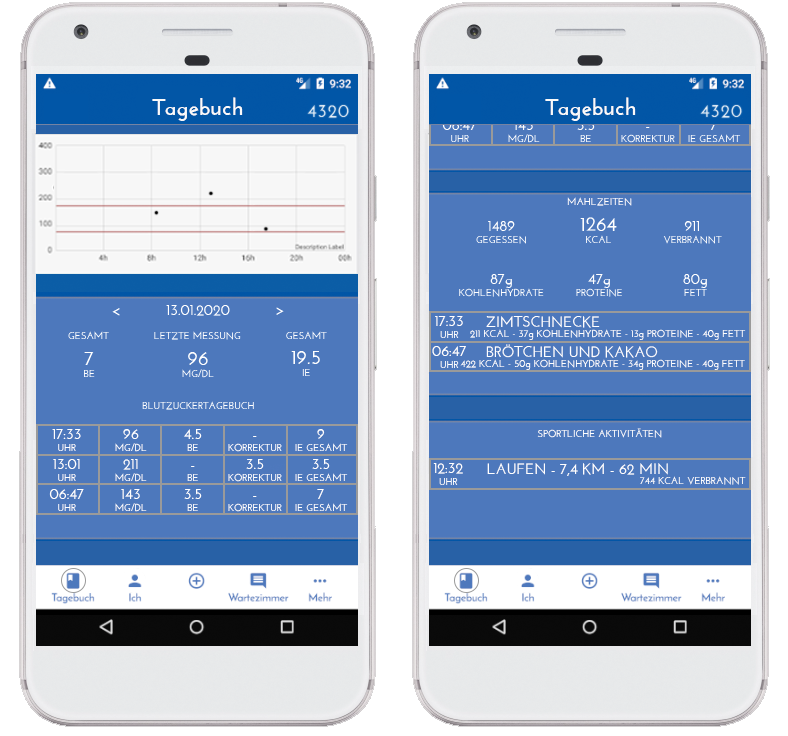
\includegraphics[width=0.66\textwidth]{images/tagebuchscreen_digital.png}
	\captionsetup{justification=centering}
	\caption{DUID: Tagebuch-Screen}
	\label{img:DUIDtagebuchscreen}
\end{figure}
In den restlichen Screens sind kaum Veränderungen zum Conceptual Model Design entstanden. Farben und Title wurden hinzugefügt, Information wurden gruppiert und voneinander abgegrenzt und Symbole und Icons wurden ausgetauscht. Im Folgenden sind die einzelnen Detailed User Inferface Designs zusehen:\\
\begin{figure}[H]
	\centering
	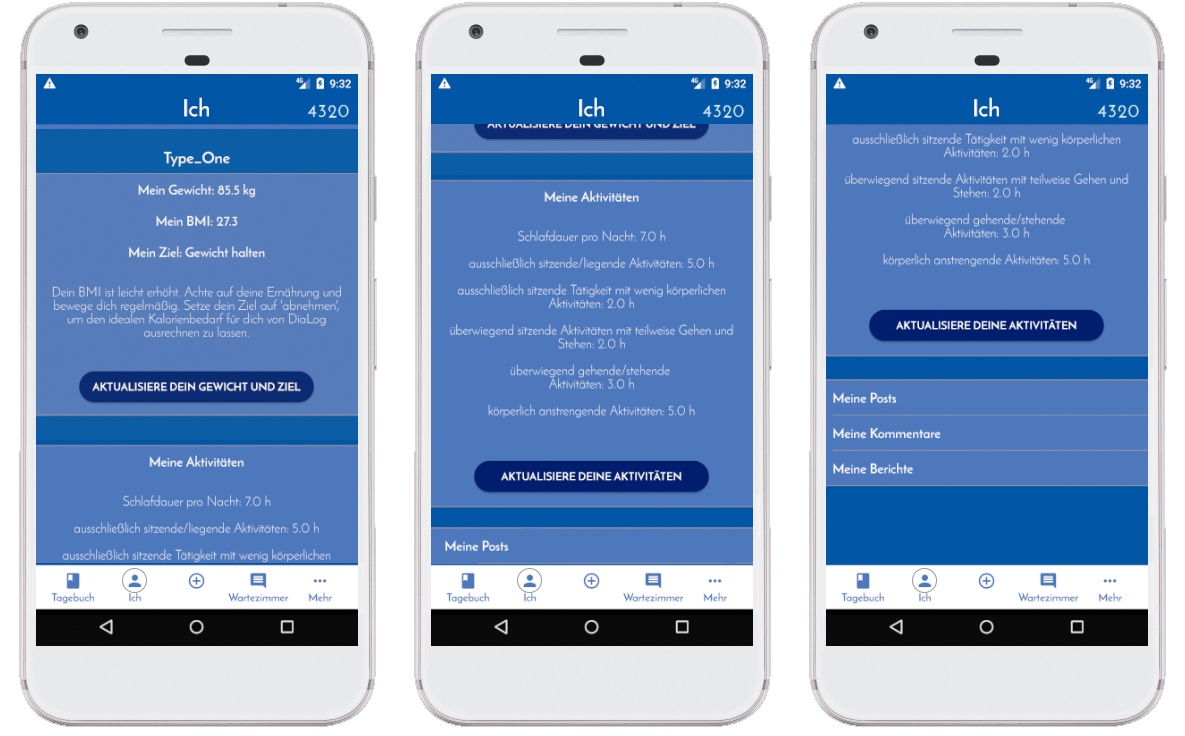
\includegraphics[width=0.99\textwidth]{images/ichscreen_digital.png}
	\captionsetup{justification=centering}
	\caption{DUID: Ich-Screen}
	\label{img:DUIDichscreen}
\end{figure}
\begin{figure}[H]
	\centering
	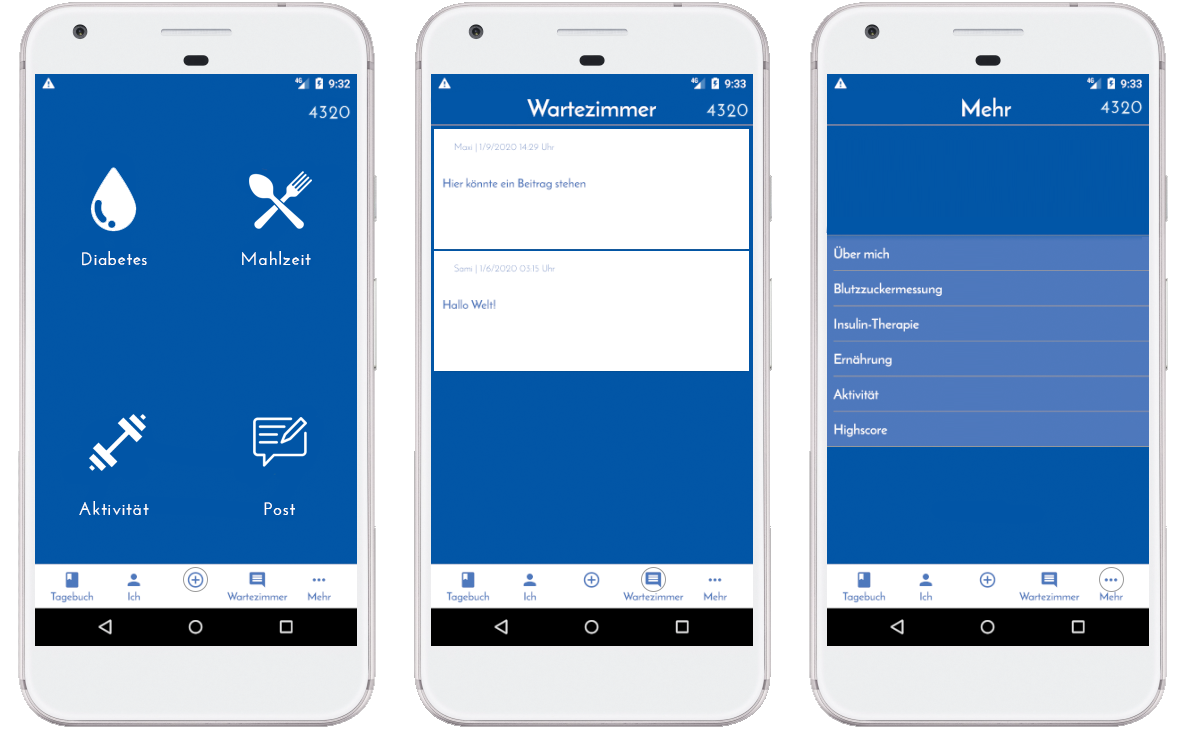
\includegraphics[width=0.99\textwidth]{images/drei_digital.png}
	\captionsetup{justification=centering}
	\caption{DUID: Add-, Wartezimmer- und Mehr-Screen (von links nach rechts)}
	\label{img:DUIdreiscreen}
\end{figure}



